\documentclass[journal]{IEEEtran}
\usepackage[utf8]{inputenc}
\usepackage[backend=biber, style=numeric, sorting=none]{biblatex}
\addbibresource{references.bib} % Add your .bib file here
\usepackage{fancyhdr}
\fancyhead{} % Clear the header and footer
\fancyfoot{}
\fancyfoot[C]{Page \thepage}
\renewcommand{\headrulewidth}{0pt} 
\pagestyle{fancy}
\usepackage{tikz}
\usetikzlibrary{shapes,backgrounds,svg.path}
\usepackage{verbatim}
\usepackage{url}
\usepackage{enumitem}
\usepackage{dirtytalk}
\usepackage{amsmath,amssymb,amsfonts}
\usepackage{xfrac}
\usepackage{algorithmic}
\usepackage{graphicx}
\usepackage{graphics}
\usepackage{svg}
\usepackage{textcomp}
\usepackage{xcolor}
\usepackage{color,soul}
\usepackage{scalerel}
\usepackage{csquotes}
\usepackage{subcaption}
\usepackage{multirow}
\usepackage[ruled,vlined]{algorithm2e}
\usepackage{nomencl}
\usepackage[hyperfootnotes=false]{hyperref}
\hypersetup{
  colorlinks,
  citecolor=black,
  linkcolor=black,
  urlcolor=black}
\makenomenclature

\newcommand{\citeauthornum}[1]{\citeauthor{#1} (\citeyear{#1}) \cite{#1}}

\newcommand{\subscript}[2]{$#1 _ #2$}

\definecolor{googleblue}{rgb}{0.259,0.522,0.957}
\definecolor{googlegreen}{rgb}{0.060,0.620,0.350}
\definecolor{googlered}{rgb}{0.859,0.267,0.220}
\definecolor{bleudefrance}{rgb}{0.19,0.55,0.91}

% begin ORCID id
\definecolor{orcidlogocol}{HTML}{A6CE39}
\tikzset{
  orcidlogo/.pic={
    \fill[orcidlogocol] svg{M256,128c0,70.7-57.3,128-128,128C57.3,256,0,198.7,0,128C0,57.3,57.3,0,128,0C198.7,0,256,57.3,256,128z};
    \fill[white] svg{M86.3,186.2H70.9V79.1h15.4v48.4V186.2z}
                 svg{M108.9,79.1h41.6c39.6,0,57,28.3,57,53.6c0,27.5-21.5,53.6-56.8,53.6h-41.8V79.1z M124.3,172.4h24.5c34.9,0,42.9-26.5,42.9-39.7c0-21.5-13.7-39.7-43.7-39.7h-23.7V172.4z}
                 svg{M88.7,56.8c0,5.5-4.5,10.1-10.1,10.1c-5.6,0-10.1-4.6-10.1-10.1c0-5.6,4.5-10.1,10.1-10.1C84.2,46.7,88.7,51.3,88.7,56.8z};
  }
}

\newcommand\orcidicon[1]{\href{https://orcid.org/#1}{\mbox{\scalerel*{

\begin{tikzpicture}[yscale=-1,transform shape]
\pic{orcidlogo};
\end{tikzpicture}
}{|}}}}
%<--- Load last for OrcidID 
% end ORCID id

\begin{document}
\raggedbottom
\onecolumn

%Title Page
\begin{titlepage}
\end{titlepage}

%table of contents
\tableofcontents
\clearpage

\twocolumn
\setcounter{page}{1}

\title{Neuro-Symbolic AI in 2024: A systematic review}

\author{
        \IEEEauthorblockN{Brandon C. Colelough,~$^{\orcidicon{0000-0001-8389-3403}}$}%
        
        \IEEEauthorblockA{School of Computer Science, University of Maryland, MD, United States}
}

\maketitle
\begingroup\renewcommand\thefootnote{\textsection}\endgroup

\begin{abstract}
abstract
\end{abstract}

\begin{IEEEkeywords}
buzz word 1, buzz word 2
\end{IEEEkeywords}

\section{Introduction} \label{sec:intro}
The field of Artificial Intelligence (AI) has experienced significant cyclical growth, known as AI summers and winters. At present, we as a community find ourselves in the third AI summer, marked by rapid scientific advances and commercialization, continuing the legacy of previous periods of AI excitement followed by setbacks \cite{Kautz2022}. A significant product of the third AI summer has been the integration of two prominent fields of AI; Symbolic AI and Sub-Symbolic AI, the fusion of which is known as neuro-symbolic AI. There is an ongoing debate about the necessity of neuro-symbolic AI \cite{Dingli2023}, with critics arguing that the world can be solved through big data and big computing and proponents arguing that \enquote{You can’t get to the moon by climbing successively taller trees} \cite{Marcus2019}. For this systematic review, we take the stance that symbolic AI is essential and that neuro-symbolic AI represents the best way forward for the community hence, this paper provides a systematic literature review of prominent neuro-symbolic projects within the 2024 AI landscape, highlighting key developments, methodologies, and applications. There has been significant interest recently in the field of neuro-symbolic AI. From a Google Scholar scraping, there has been a total of 945 publications, with notable increases in the years beginning from 2020 (53 publications), and peaking in 2023 (280 publications).

\begin{figure}[ht]
    \centering
   \includesvg[width=0.6\textwidth]{Figures/publications_by_year.svg}
    \caption{Number of publications per year for neuro-symbolic AI. The data was obtained through Google Scholar scraping, reflecting significant growth from 2020}
    \label{fig:pubs_by_year}
\end{figure}

\subsection{Neuro-symbolic AI: A Definition}

\subsubsection{\textbf{Symbolic AI}}\label{subsub:symbolic-AI}
As described by \citeauthornum{Dingli2023}, Symbolic AI is a \enquote{a sub-field of AI concerned with learning the internal symbolic representations of the world around it} where we can \enquote{ translate some form of implicit human knowledge into a more formalized and declarative form based on rules and logic}. Examples of some of the earliest AI systems that utilised symbolic representations include SHRDLU from \citeauthornum{SHRDLU}, ELIZA from \citeauthornum{Weizenbaum1966},  DENDRAL from \citeauthornum{Lindsay1980} and MYCIN from \citeauthornum{Melle1978} and examples of some of the newest AI systems which heavily utilise symbolic processes include ConceptNet 5.5 by \citeauthornum{Speer2016} CYC from \citeauthornum{Lenat2023} and Good Old Fashioned AI (GOFAI) planning systems as described by \citeauthornum{Edelkamp2004} to name just a few.

\subsubsection{\textbf{Sub-Symbolic AI}}
By contrast, Sub-symbolic-AI, as again described by \citeauthornum{Dingli2023} are systems that \enquote{do not require rules or symbolic representations as inputs} and instead \enquote{learn implicit data representations on their own}. Sub-symbolic AI encompasses approaches such as machine learning, deep learning, and generative AI etc., which rely on algorithms to automatically extract patterns from raw data to discern relationships and make predictions based on learned representations. Examples of some of the earliest AI systems that utilised sub-symbolic representations include the Perceptron developed by \citeauthornum{Rosenblatt1958}, Hopfield Networks developed by \citeauthornum{Hopfield1982} and the Backpropagation Algorithm Formulated by \citeauthornum{Rumelhart1986} and examples of some of the newest sub-symbolic systems include famous projects such as the Generative Pre-trained Transformer (GPT) models by \citeauthornum{Vaswani2017}, the YOLO family of Convolutional Neural Networks (CNN'S) by \citeauthornum{Redmon2015} and the DALLE diffusion model transformer from \citeauthornum{Ramesh2021} to again just name a few. Figure \ref{fig:sub-and-symbolic-AI} below shows the difference between symbolic and sub-symbolic AI and how symbolic representations can emerge from sub-symbolic processes to be subsequently mapped to a symbolic feature map. 

\begin{figure}[ht]
    \centering
    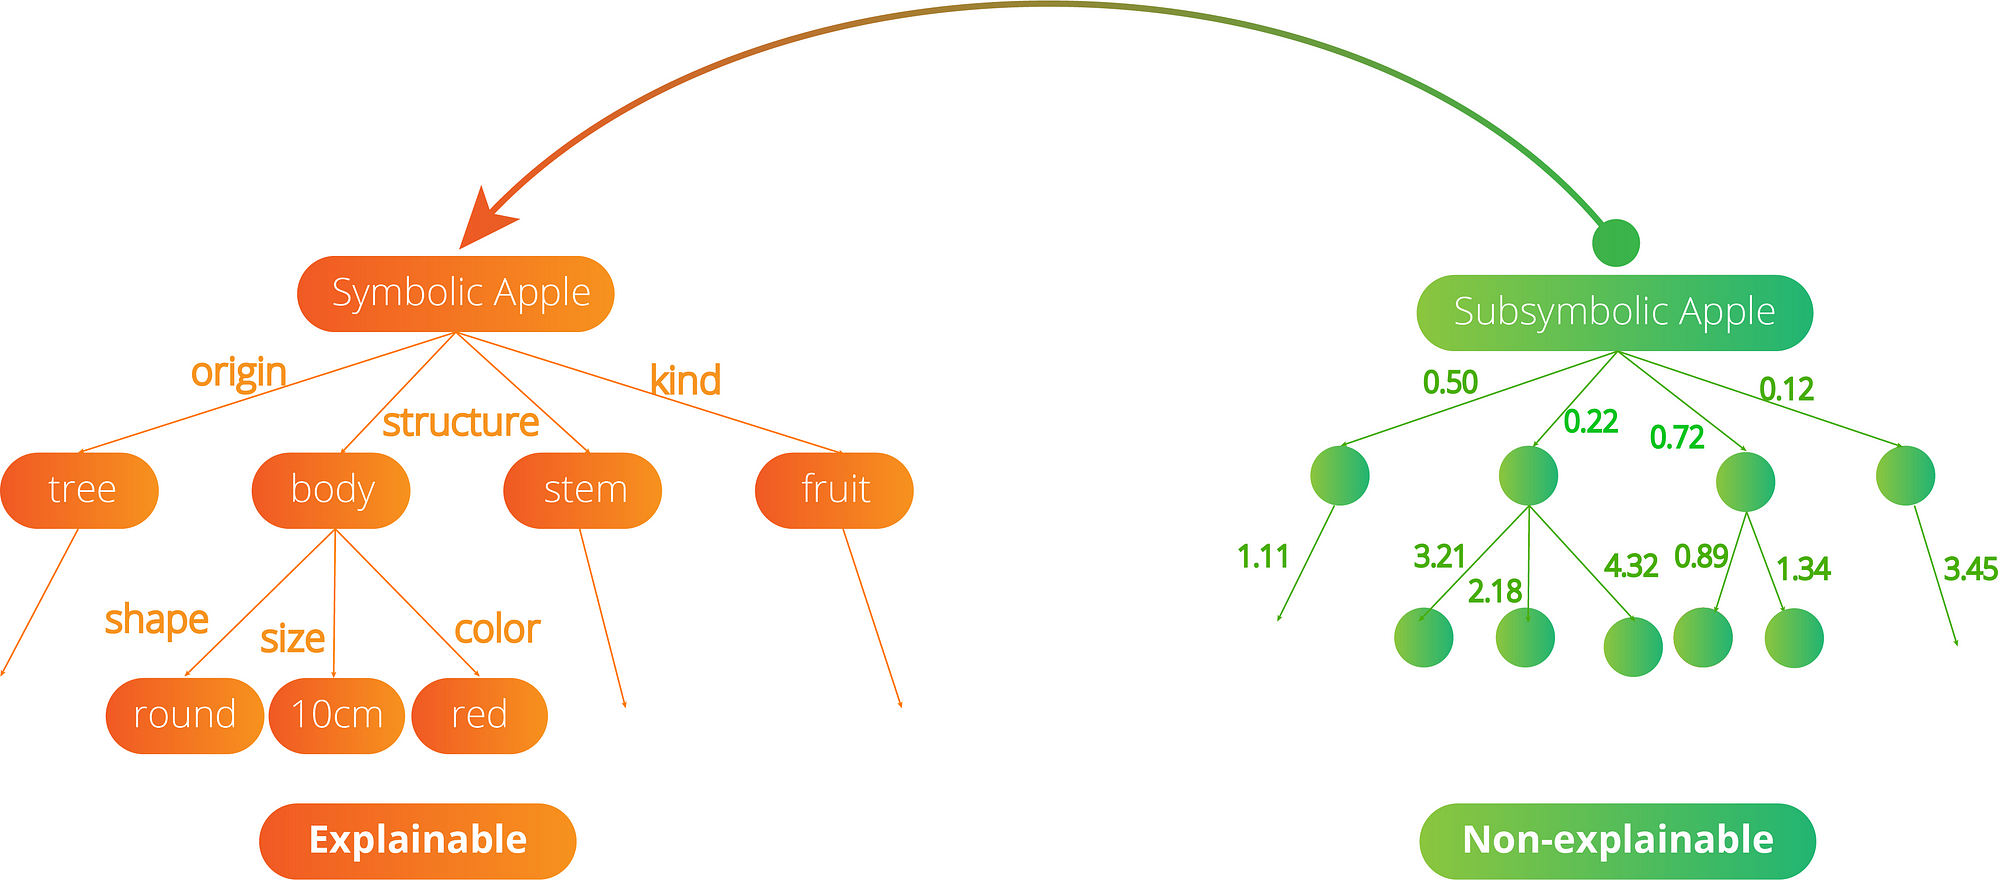
\includegraphics[width=\textwidth/2]{Figures/Symbolic_VS_SubSymbollic_AI.png}
    \caption{The above figure, taken from \cite{Yalcin2021},  contrasts Symbolic AI (left, Orange), which represents knowledge in a human-understandable format (hierarchically chained with suitable sub-components such as tree, body, colour), with Sub-Symbolic AI (right, green), which uses numerical weights and connections, making it harder to interpret directly. The arrow from sub-symbolic to symbolic in the above picture represents how symbolic representations can be derived from sub-symbolic data}
    \label{fig:sub-and-symbolic-AI}
\end{figure}


\subsubsection{\textbf{Daniel Kahneman with System 1 and System 2 thinking}}
As explored by \citeauthornum{Garcez2023}, there is at present a debate within the AI community surrounding the need for neuro-symbolic AI. Simply described, the argument for neuro-symbolic AI draws on \citeauthornum{Kahneman2011} concepts of System 1 and System 2 thinking whereby System 1 is fast, intuitive, and parallel, akin to the capabilities of deep learning, while System 2 is slow, deliberate, and sequential, resembling symbolic reasoning and hence, neuro-Symbolic AI aims to combine these two approaches to create systems that benefit from the strengths of both. As will be explored in section \ref{sec:discussion}, it is our opinion that whilst this initial representation of neuro-symbolic AI is a useful tool to goal-orientate the field towards a common direction for the integration of neural and symbolic processes, the current adaptation of the human-level cognitive processing ability is too simplistic and does not yet capture the full systems level breakdown of where the community should be investing effort to push the field forward.  

\subsubsection{\textbf{Neuro-symbolic AI}}
To clearly define exactly what we mean by the term neuro-symbolic AI, we rely on the definition provided by \citeauthornum{Garcez2023}; Hence, Neuro-symbolic AI is \textbf{\enquote{a composite AI framework that seeks to merge the domains of Symbolic AI and NNs} [or more broadly put, Sub-Symbolic AI] \enquote{to create a superior hybrid AI model possessing reasoning capabilities}}. As this definition is quite broad, for the purpose of this systematic review, we will further define the sub-components of the Neuro-Symbolic AI Spectrum we believe to be most relevant to the current AI landscape within section \ref{sec:methodology}. 


\section{Methodology}\label{sec:methodology}
A manual search process was conducted to identify published peer-reviewed articles. This process followed the \href{https://www.prisma-statement.org/}{PRISMA} systematic review methodology and utilised the following databases:


\begin{enumerate}
    \item \href{https://ieeexplore.ieee.org/Xplore/home.jsp}{IEEE Explore}
    \item \href{http://scholar.google.com}{Google Scholar}
    \item \href{https://arxiv.org/}{arxiv online library}
    \item \href{http://portal.acm.org/portal.cfm}{The Association for Computing Machinery (ACM) }
    \item \href{http://www.springerlink.com}{SpringerLink Library}
\end{enumerate}


First, an initial search was conducted to identify relevant systematic reviews and survey papers for the field of neuro-symbolic artificial intelligence through querying the paper title information. Only peer-reviewed papers published between 2022-2024 were considered. Results of this initial survey are shown in table \ref{tab::hits_results}. The results were further screened to remove duplicates and papers that were not relevant to the broad application space of neurosymbolic AI. The following 6 survey papers on the field of neuro-symbolic AI were then selected; \citeauthornum{Gibaut2023},  \citeauthornum{Yu2021}, \citeauthornum{Wan2024}, \citeauthornum{Marra2024}, \citeauthornum{MichelDeletie2024}, \citeauthornum{Bouneffouf2022}. The 6 selected survey papers were then used in conjunction with the following 4 books by \citeauthornum{Dingli2023}, \citeauthornum{Hitzler2023} and \citeauthornum{Hitzler2021} and \citeauthornum{Shakarian2023} to synthesize the following research question, search criteria and accept/reject criteria for the systematic literature review: 

\subsection{Research question}\label{subsec:research_quest}
\textbf{"Within the major sub-fields of neuro-symbolic AI, where is the quality of effort being focused in 2024, and what are the existing research gaps in the current literature?"}

\subsection{The Neuro-Symbolic AI Spectrum}
To answer the above question, we first identified from the 6 survey papers and 4 books, the major sub-fields of neuro-symbolic AI. 7 foundational research areas were thus distilled from these 10 pieces of literature. The foundational research areas for neuro-symbolic AI, synthesized from the work of various researchers, include: 
\begin{enumerate}
    \item \textbf{Knowledge Representation}, which involves integrating symbolic and neural representations as well as developing commonsense and domain-specific knowledge graphs \cite{Gibaut2023, Hitzler2023, Shakarian2023};
    \item \textbf{Learning and Inference}, focusing on combining learning and reasoning processes through end-to-end differentiable reasoning and dynamic multi-source knowledge reasoning \cite{Yu2021, Wan2024, Dingli2023};
    \item \textbf{Explainability and Trustworthiness}, which aims to create interpretable models and reasoning processes to ensure trust and reliability in neuro-symbolic systems \cite{Marra2024, MichelDeletie2024};
    \item \textbf{Logic and Reasoning}, integrating logic-based methods with neural networks, including logical and probabilistic reasoning and the syntax and semantics of neuro-symbolic systems \cite{Marra2024, Shakarian2023};
    \item \textbf{Meta-level Cognition} involves the system's capacity to monitor, evaluate, and adjust its own reasoning and learning processes by integrating neural networks and symbolic representations.

\end{enumerate}

The above categories represent the core technical areas where current efforts are concentrated from the literature skim of survey papers and currently available books on neurosymbolic AI. There is, however, an extra category, meta-level cognition, that we are adding that was not present in the literature as we believe it will be important for the field going forward. 

\subsection{PRISMA Search Criteria}
\begin{itemize}
    \item \textbf{Keywords}: Neurosymbolic AND [Knowledge Representation, Reasoning learning, inference, explainability, trustworthiness, architectures, logic, formal methods, applications, challenges].
    \item \textbf{Publication Years}: 2022-2024.
    \item \textbf{Document Types}: Peer-reviewed journal articles, conference papers, survey papers, systematic reviews, and books.
    \item \textbf{Language}: English.
    \item \textbf{Search Area}: Title only (Abstract for Springer)
\end{itemize}

\subsection{Accept/Reject Criteria}
\begin{itemize}
    \item \textbf{Inclusion Criteria}:
    \begin{itemize}
        \item Papers published between 2020 and 2024.
        \item Articles addressing any of the seven foundational research areas.
        \item Peer-reviewed and academic sources.
    \end{itemize}
    \item \textbf{Exclusion Criteria}:
    \begin{itemize}
        \item Papers published before 2020.
        \item Papers not in English
        \item Survey / systematic review papers 
        \item Non-peer-reviewed articles, such as editorials, opinions, or preprints not peer-reviewed.
        \item Articles not addressing the specified sub-fields of neuro-symbolic AI.
        \item Duplicate entries.
        \item Any paper that had an associated codebase that was not made publicly available (i.e. non-reproducible projects)
    \end{itemize}
\end{itemize}

\subsection{Screening Methodologies}
A broad search was conducted using the identified keywords across selected databases to query the literature title (title and abstract for Springer database as the title alone gave no results), and all search results were imported into JabRef. The number of records identified from each database was documented as. Duplicate records were then identified and removed using JabRef. Titles and abstracts of the collected papers were screened to assess relevance based on the inclusion and exclusion criteria, categorizing papers into "Include," "Exclude," or "Uncertain." Full texts of papers categorized as "Include" or "Uncertain" were retrieved and reviewed, rigorously applying the inclusion and exclusion criteria to determine the final list of papers to be included in the review. Data were extracted from the selected papers, including authors and publication year, title and source, major research areas addressed, and key findings relevant to the research question. The extracted data were organized into the seven foundational research areas, identifying and summarizing the quality of effort and existing research gaps within each area.

\section{Results}\label{sec:results}

\begin{figure*}[ht]
    \centering
    \resizebox{\textwidth}{!}{

    \begin{tabular}{ |p{3cm}||p{6cm}|p{6cm}|}
     \hline
     \multicolumn{3}{|c|}{Survey Paper findings for Neuro-symbolic AI} \\
     \hline
    Database &"neurosymbolic" AND "systematic review" &  "neurosymbolic" AND "survey" \\
     \hline
     IEEE   & 0 & 2 \\
     Google Scholar & 2 & 10 \\
     ArXiv & 0 & 8 \\
     ACM  & 1 & 4 \\
     Springer & 0 & 0\\
     \hline
    \end{tabular}

    }

\captionof{table}[Hits_Results]{The search terms "neurosymbolic" AND "systematic review" and "neurosymbolic" AND "survey" were queried through the 5 databases. The number of pieces of literature returned from each query is shown in the table above. Note also that only publications from 2022-2024 were considered}
\label{tab::hits_results}
\end{figure*}

\begin{figure*}[ht]
    \centering
    \resizebox{\textwidth}{!}{
    \begin{tabular}{|p{3cm}||p{3cm}|p{3cm}|p{3cm}|p{3cm}|p{3cm}|}
        \hline
        \multicolumn{6}{|c|}{Article Findings for Neuro-symbolic AI within the 5 foundational areas of research} \\
        \hline
        Database & Knowledge & Learning, Inference & Explainability, Trustworthiness & Logic, Reasoning & Meta-Level, Cognition \\
        \hline
        IEEE & 73 & 97 & 15 & 67 & 33  \\
        Google Scholar & 56 & 126 & 7 & 129 & 3  \\
        ArXiv & 17 & 54 & 7 & 55 & 3  \\
        ACM & 10 & 46 & 5 & 12 & 17  \\
        Springer & 152 & 170 & 65 & 162 & 47  \\
        Total(after screening)   & 308 & 493 & 99 & 425 & 103  \\
        \hline
     \end{tabular}

    }

\captionof{table}[Hits_Results]{The search terms "neurosymbolic" AND each of the terms required for the 5 foundational research areas within neurosymbolic AI were queried through the 5 databases. The number of pieces of literature returned from each query is shown in the table above. Note also that only publications from 2020-2024 were considered}
\label{tab::hits_results}
\end{figure*}

%%%%%%%%%%%%%%%%%%%%%%%%%%%%%%%%%%%%%%%%%% VENN Diagram

\def\firstcircle{(-1.5,1.5) circle (3cm)}
\def\secondcircle{(1.5,1.5cm) circle (3cm)}
\def\thirdcircle{(1.5,-1.5cm) circle (3cm)}
\def\fourthcircle{(-1.5,-1.5cm) circle (3cm)}

\begin{figure*}[ht]
    \centering
    \resizebox{\textwidth}{!}{

    % Now we can draw the sets:
    \begin{tikzpicture}

        % The last trick is to cheat and use transparency
        \begin{scope}[shift={(-4cm,0cm)}, fill opacity=0.5]
            \fill[red] \firstcircle;
            \fill[green] \secondcircle;
            \fill[blue] \thirdcircle;
            \fill[yellow] \fourthcircle;
            \draw \firstcircle node[above] {};
            \draw \secondcircle node [above] {};
            \draw \thirdcircle node [above] {};
            \draw \fourthcircle node [below] {};
        \end{scope}
    \node at (-7,3) {\textbf{Logic and }};
    \node at (-7,2.5) {\textbf{Reasoning }};
    
    \node at (-1.5,3) {\textbf{Learning and }};
    \node at (-1.5,2.5) {\textbf{Inference}};
    
    \node at (-6.5,-3) {\textbf{Explainability and }};
    \node at (-6.5,-3.5) {\textbf{Trustworthiness}};

    \node at (-1.5,-3) {\textbf{Knowledge}};
    \node at (-1.5,-3.5) {\textbf{Representation}};

    % references within VENN diagrams
    \tiny

        %Middle
        \node at (-4.5, 0) {\textbf{\cite{TOSM}}};
        \node at (-4, 0) {\textbf{\cite{TOSM}}};
        \node at (-3.5, 0) {\textbf{\cite{TOSM}}};
        \node at (-4.2, -0.5) {\textbf{\cite{TOSM}}};

        %4. Logic and Reasoning
        \node at (-8,2) {\textbf{\cite{TOSM}}};
        \node at (-7.5,2) {\textbf{\cite{TOSM}}};
        \node at (-7,2) {\textbf{\cite{TOSM}}};
        \node at (-6.5,2) {\textbf{\cite{TOSM}}};
        \node at (-6,2) {\textbf{\cite{TOSM}}};
        \node at (-8, 1.5) {\textbf{\cite{TOSM}}};
        \node at (-7.5, 1.5) {\textbf{\cite{TOSM}}};
        \node at (-7, 1.5) {\textbf{\cite{TOSM}}};
        \node at (-6.5, 1.5) {\textbf{\cite{TOSM}}};
        \node at (-6, 3) {\textbf{\cite{TOSM}}};
        \node at (-7, 3.5) {\textbf{\cite{TOSM}}};
        \node at (-6.5, 3.5) {\textbf{\cite{TOSM}}};
        \node at (-6, 3.5) {\textbf{\cite{TOSM}}};

        %Logic int explain int knowledge
        \node at (-5, -1) {\textbf{\cite{TOSM}}};

        %Logic int learning int knowledge representation
        \node at (-3.5, 1) {\textbf{\cite{TOSM}}};

        %Logic int explain
        \node at (-7.5, 0) {\textbf{\cite{TOSM}}};
        \node at (-7, 0) {\textbf{\cite{TOSM}}};

        %Logic int learning
        \node at (-5, 2) {\textbf{\cite{TOSM}}};
        \node at (-4.5, 2) {\textbf{\cite{TOSM}}};
        \node at (-4, 2) {\textbf{\cite{TOSM}}};
        \node at (-3.5, 2) {\textbf{\cite{TOSM}}};

        %Logic int learning int explain
        \node at (-5, 1) {\textbf{\cite{TOSM}}};

        %learning
        \node at (-1,2) {\textbf{\cite{TOSM}}};
        \node at (-1.5,2) {\textbf{\cite{TOSM}}};
        \node at (-2,2) {\textbf{\cite{TOSM}}};
        \node at (-0.5,2) {\textbf{\cite{TOSM}}};
        \node at (0,2) {\textbf{\cite{TOSM}}};
        \node at (-0.5, 2.5) {\textbf{\cite{TOSM}}};

        %knowledge representation
        \node at (-1.5, -1.5) {\textbf{\cite{TOSM}}};
        \node at (-1, -1.5) {\textbf{\cite{TOSM}}};
        \node at (-.5, -1.5) {\textbf{\cite{TOSM}}};
        \node at (0, -1.5) {\textbf{\cite{TOSM}}};

        %%newline

        \node at (-2, -2) {\textbf{\cite{TOSM}}};
        \node at (-1.5, -2) {\textbf{\cite{TOSM}}};
        \node at (-1, -2) {\textbf{\cite{TOSM}}};
        \node at (-0.5, -2) {\textbf{\cite{TOSM}}};
        \node at (0, -2) {\textbf{\cite{TOSM}}};

        %%newline

        \node at (-2, -2.5) {\textbf{\cite{TOSM}}};
        \node at (-1.5, -2.5) {\textbf{\cite{TOSM}}};
        \node at (-1, -2.5) {\textbf{\cite{TOSM}}};
        \node at (-.5, -2.5) {\textbf{\cite{TOSM}}};
        \node at (0, -2.5) {\textbf{\cite{TOSM}}};

        %%newline

        \node at (-2.7, -4) {\textbf{\cite{TOSM}}};
        \node at (-3.2, -4) {\textbf{\cite{TOSM}}};
        \node at (-2.2, -4) {\textbf{\cite{TOSM}}};
        \node at (-1.7, -4) {\textbf{\cite{TOSM}}};
        \node at (-1.2, -4) {\textbf{\cite{TOSM}}};

        %knowledge representation int explain
        \node at (-5, -2) {\textbf{\cite{TOSM}}};
        \node at (-4.5, -2) {\textbf{\cite{TOSM}}};
        \node at (-4, -2) {\textbf{\cite{TOSM}}};
        \node at (-3.5, -2) {\textbf{\cite{TOSM}}};
        \node at (-3, -2) {\textbf{\cite{TOSM}}};

        %explain
        \node at (-8,-2) {\textbf{\cite{TOSM}}};
        \node at (-7.5, -2) {\textbf{\cite{TOSM}}};
        \node at (-7, -2) {\textbf{\cite{TOSM}}};
        \node at (-6.5, -2) {\textbf{\cite{TOSM}}};
        \node at (-6, -2) {\textbf{\cite{TOSM}}};
        \node at (-8, -2.5) {\textbf{\cite{TOSM}}};

        %knowledge representation int learning
        \node at (-0.5,0) {\textbf{\cite{TOSM}}};
        \node at (-1,0) {\textbf{\cite{TOSM}}};
        \node at (-1.5,0) {\textbf{\cite{TOSM}}};
        \node at (-2,0) {\textbf{\cite{TOSM}}};
        \node at (-2.5, 0) {\textbf{\cite{TOSM}}};

        %%%newline

        \node at (-0.7, -.5) {\textbf{\cite{TOSM}}};
        \node at (-1.2, -0.5) {\textbf{\cite{TOSM}}};
        \node at (-1.7, -0.5) {\textbf{\cite{TOSM}}};

        %%%newline

        \node at (-0.7, 0.5) {\textbf{\cite{TOSM}}};
        \node at (-1.2, 0.5) {\textbf{\cite{TOSM}}};
        \node at (-1.7, 0.5) {\textbf{\cite{TOSM}}};
        \node at (-2.2, 0.5) {\textbf{\cite{TOSM}}};

        %%newline

        \node at (-1.2, 1) {\textbf{\cite{TOSM}}};
        \node at (-1.7, 1) {\textbf{\cite{TOSM}}};
        \node at (-2.2, 1) {\textbf{\cite{TOSM}}};

        %explain int knowledge representation int learning
        \node at (-3.5, -1) {\textbf{\cite{TOSM}}};
        \node at (-3, -1) {\textbf{\cite{TOSM}}};
        \node at (-2.9, -0.5) {\textbf{\cite{TOSM}}};

        \normalsize
        \node at (-6,-5){\textbf{Meta-Level Cognition}};
        \tiny
        \draw (0,-5.5) -- (-8,-5.5) -- (-8,-7) -- (0,-7) -- (0,-5.5);
        \node at (-7.5,-6)  {\textbf{\cite{TOSM}}};
        \node at (-7,-6) {\textbf{\cite{TOSM}}};
        \node at (-6.5,-6) {\textbf{\cite{TOSM}}};
        \node at (-6, -6) {\textbf{\cite{TOSM}}};
        \node at (-5.5, -6) {\textbf{\cite{TOSM}}};
        \node at (-5, -6) {\textbf{\cite{TOSM}}};
        \node at (-4.5, -6) {\textbf{\cite{TOSM}}};
        \node at (-4, -6) {\textbf{\cite{TOSM}}};
        \node at (-3.5, -6) {\textbf{\cite{TOSM}}};
        \node at (-3, -6) {\textbf{\cite{TOSM}}};
        \node at (-2.5, -6) {\textbf{\cite{TOSM}}};
        \node at (-2,-6)  {\textbf{\cite{TOSM}}};
        \node at (-1.5,-6) {\textbf{\cite{TOSM}}};
        \node at (-1, -6) {\textbf{\cite{TOSM}}};
        \node at (-0.5,-6) {\textbf{\cite{TOSM}}};
        

    \end{tikzpicture}
}
\caption{A literature review of existing of the major components of Symbolic AI was conducted}
\label{fig::venn_diagram}
\end{figure*}

%%%%%%%%%%%%%%%%%%%%%%%%%%%%%%%%%%%%%%%%%% VENN Diagram


\section{Discussion}\label{sec:discussion}

\subsection{Cognition within Neuro-symbolic AI}
\subsubsection{The Common Model of Cognition}
The Common Model of Cognition (CMC), initially introduced as the Standard Model of the Mind by \citeauthornum{Laird2017}, provides a unified framework that encapsulates the fundamental architectural principles of human cognition. This model integrates key cognitive components such as perception, working memory, motor functions, declarative memory, and procedural memory, reflecting a consensus among various cognitive architectures like Adaptive Control of Thought-Rational (ACT-R), State, Operator, And Result (Soar), and Sigma. 

The integration of cognitive architectures with foundation models is further elaborated by \citeauthornum{Thomson2024}, who discusses cognitively guided few-shot learning to support trusted AI. This integration aims to combine the strengths of cognitive models with the data-driven capabilities of foundation models, thereby enhancing the robustness and interpretability of AI systems. \citeauthornum{West2024} further explores bridging generative networks with the CMC, emphasizing the potential of combining symbolic reasoning with neural networks. This neuro-symbolic approach leverages the strengths of both paradigms, offering a comprehensive method to replicate human cognitive processes. Such integration is crucial for developing advanced AI systems that are both powerful and explainable. By aligning the principles of the CMC with modern AI techniques, neuro-symbolic AI can achieve a more holistic understanding and replication of human cognition, paving the way for more robust and trustworthy AI systems. This paper serves as a systematic literature review of prominent neuro-symbolic projects within the 2024 AI landscape, highlighting key developments and methodologies in this interdisciplinary field.


\section{Conclusion}\label{sec:conclusion}

\clearpage
\printbibliography

\onecolumn
\clearpage

\begin{appendices}
\section{Supplementary Materials}

\nomenclature{\(O\)}{Ontology}
\nomenclature{\(\)}{}

\printnomenclature

\end{appendices}

\end{document}
